% !TeX root = ../thesis.tex

\chapter{Methodology}
\label{sec:methodology}

This chapter aims to describe the methodology adapted for generating panoptic segmentation. First section provides details about a structured approached employed to generate class-agnostic instance masks from predicted center points and offset vectors. Subsequently, it describes highly efficient merging operation between semantic and instance semantic segmentation to generate a unified and coherent panoptic scene representation.

\bigskip

\section{Approach}

 To generate a coherent and comprehensive representation of the environment under observation, it is desired to have a representation that not only describes semantic layout of the environment but also provides instance-level information on traffic participants. Further, it is desired to have a single representation that encodes both modalities and provides for a simple pixel-level expression of class label and instance id. By doing so, pixel-level fine-grained segregation of the scene can be achieved. To this end, a structured approach has been adapted to combine network predictions to achieve such a unified representation i.e. panoptic scene segmentation. General approach adopted for this purpose can be seen in the figure  \ref{fig:panoptic_seg_approach}. In figure \ref{fig: panopticdeeplab_diag}, it can be seen that the implemented network architecture adopts dual-decoder structure one for learning instance segmentation while the other learns pixel relationships. Furthermore, instance decoder is extended by two task specific heads for center point predictions and offset vectors predictions. In the first step, task specific outputs in instance decoder (center predictions and offset predictions) are combined to generate class-agnostic instance masks which makes use of a simple regression operation. Subsequently, the generated instance segmentation and semantic segmentation prediction from both decoders are combined. In the first step however, both predicted representations from instance decoder are pre-processed before the merging operation could begin. This has been explained in more detail in following sections independently for each prediction.

\begin{figure}[!ht]
    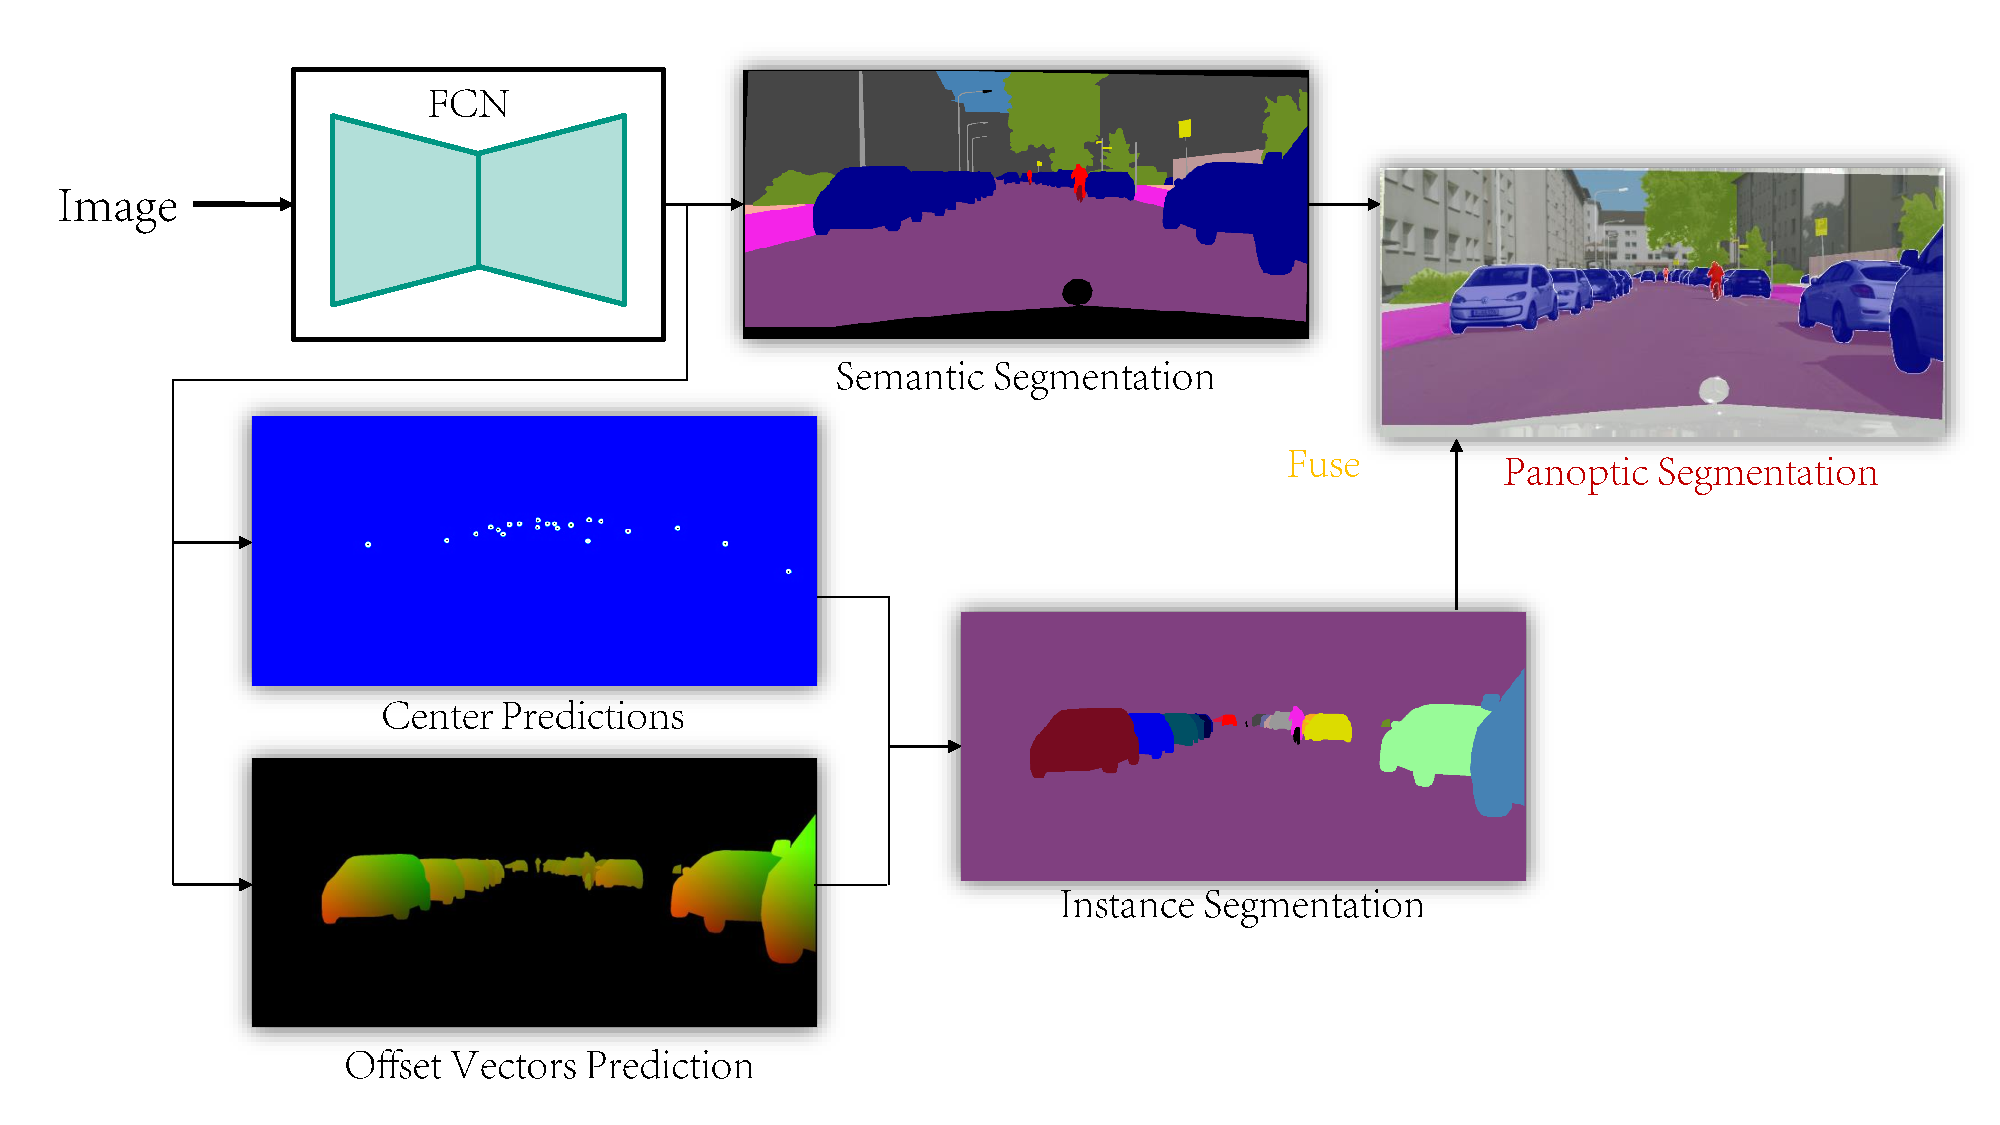
\includegraphics[width = \textwidth]{Graphics/Methodology/panoptic_seg_approach.pdf}
    \caption[Panoptic Segmentation Approach]{Illustration of general approach for panoptic segmentation - showing \gls{fcn} predicting 3 outputs where center points are offset representations combine to generate instance segmentation which in turn combines with semantic segmentation to generate panoptic segmentation.}
    \label{fig:panoptic_seg_approach}
\end{figure}


\subsection{Center Rendering}
\label{subsec:center_rendering}

During inference, center point predictions are pre-processed primarily for extracting exact center point locations out of center prediction (which is a probability distribution around center points). Furthermore, it is also desired to do a non-maxima suppression to avoid any false positives that might appear. Since, task specific head for center-point predictions is trained against a representation containing probability distributions around center-points of each \textit{things} class instance, therefore the output predicted by trained network also predicts a similar representation of probability distributions around probable center-points. Therefore, before a hough voting based grouping operation similar to \cite{Ballard1981} could be employed to generate class-agnostic instance segmentation, it is desired to extract exact pixel locations for each center point. 
To render exact center location and suppressing any false positives, following steps are performed:

\begin{enumerate}
    \item Threshold based non-maxima suppression.
    \item Max-pooling based non-maxima suppression.
    \item Filtering top-k number of pooled centers.
\end{enumerate}


\begin{figure}[!ht]
%\centering
    \subfigure[Predicted heatmap]{
        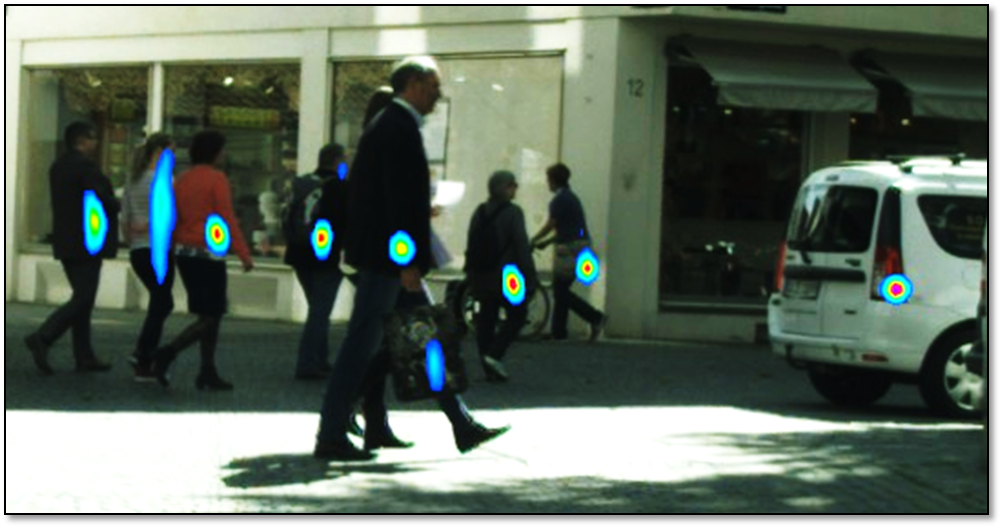
\includegraphics[width = \textwidth / 2 ]{Graphics/Methodology/Picture1}
        \label{fig:centerrawpred}}
    %\hspace{1pt}
     %add desired spacing between images, e. g. ~, \quad, \qquad, \hfill etc.
     %(or a blank line to force the subfigure onto a new line)
    \subfigure[Scaled and threshold at 0.39]{
        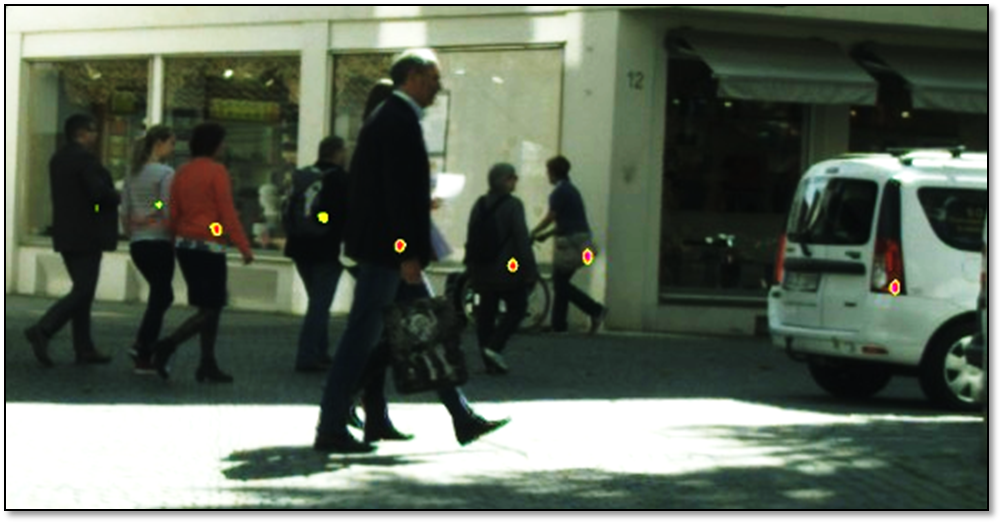
\includegraphics[width = \textwidth / 2 ]{Graphics/Methodology/Picture2}
        \label{fig:centerthreshold}}
    \subfigure[Max-pooling based NMS]{
        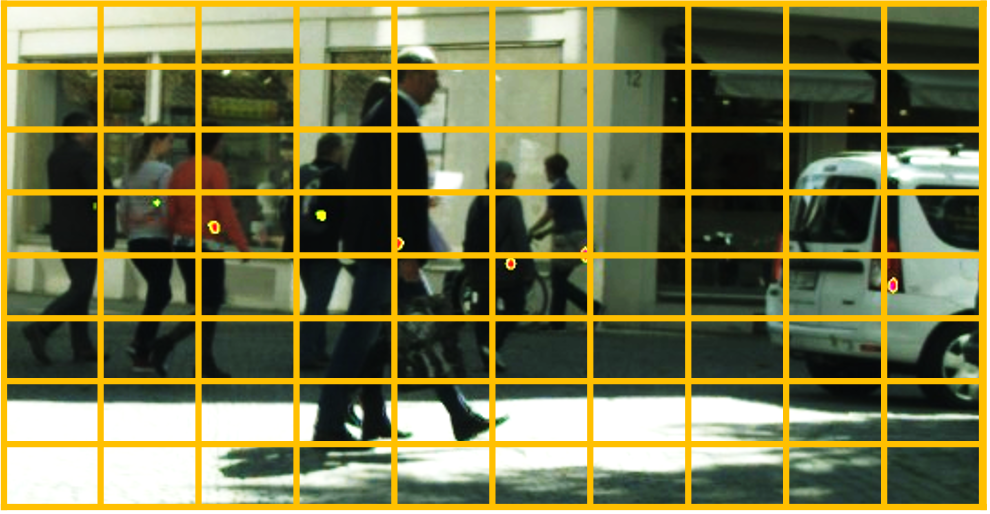
\includegraphics[width = \textwidth / 2 ]{Graphics/Methodology/Picture3}
        \label{fig:centermaxthreshold}}
%   \hspace{1pt}
    \subfigure[Extracted center locations]{
        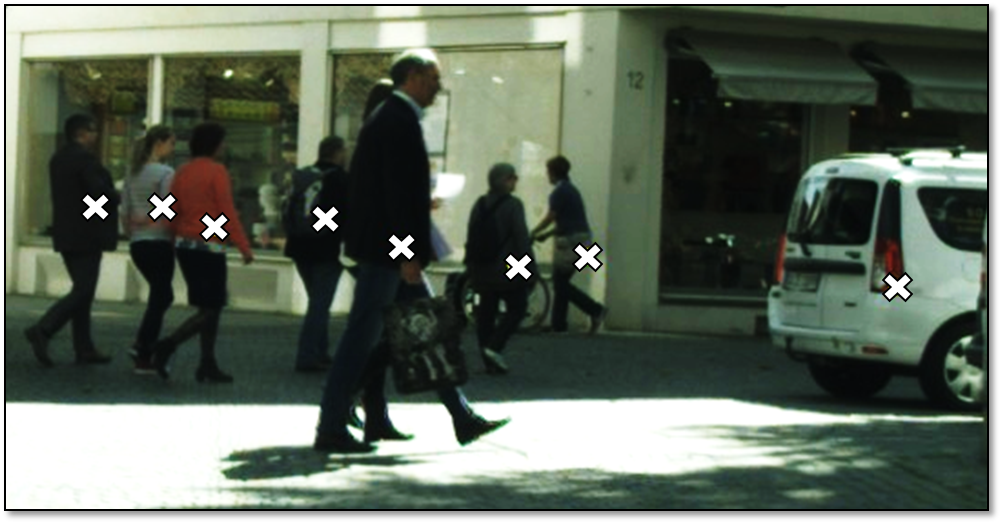
\includegraphics[width = \textwidth / 2 ]{Graphics/Methodology/Picture4}
        \label{fig:center_extracted}}
    \caption[Center Position Extraction ] {Raw center predictions from the network and subsequent steps for non-maxima supression and extracting exact center positions a) depicts raw predicted heatmap with centers represented by a probability distribution b) shows scaled and thresholded heatmap c) shows a non-maxima suppression (NMS) based on max-pooling with a fixed kernel window d) shows exact center locations extracted using max-pooling by keeping only highest prediction location in each kernel window.}
    \label{fig:centerpred_preprocessing}
\end{figure}

Center point prediction head in the network predicts a representation where each center point has been predicted as a probability distribution around probable center, visualisation of such output from network can be seen in figure \ref{fig:centerrawpred} where each distribution can be seen to extend over a number of pixels. It is desired to extract an exact number of center points with accurate locations. To this end, first the probabilities are scaled between $0-1$ and thresholded at $0.39$ , see figure \ref{fig:centerthreshold}. It was found that thresholding at $0.39$ resulted in acceptable trade-off between false positives and false negatives.   This is followed by a non-maxima suppression step which has been implemented efficiently as a max-pooling operation with stride of a single pooling window by keeping only the location of pixel with highest prediction confidence in each window as shown in figure \ref{fig:centermaxthreshold}, for further information see section \ref{subsec: pooling_operation}. This results in an effective non-maxima suppression resulting in unique center point locations which can be used for grouping offset representations to their corresponding centers. Additionally, maximum number of center-points are restricted to a highest of 200. Therefore, picking only the top-k center points from pooled centers where k in this case is chosen to be 50 or 200. The resulting center points after these operations are used for grouping offset vectors.




\subsection{Offset Directions}

In chapter \ref{sec:data_representation}, information about various data representations has been provided. In this work, various representations and encoding were conceptualized and implemented to generate datasets that were used to train the network. Section \ref{subsec:offsets}, describes few offset representation possibilities that are well-suited for representing pixel relationships to their center points. More specifically, it can be seen that end-to-end encoding can directly encode the distance and direction i.e. real offset with direction information required to reach its center point, see figure \ref{fig:e2e_vis_pixels}. On the other hand, center-to-end encoding only encodes the distance i.e  offset in terms of magnitude that is required to reach center without encoding direction, as visualised in figure \ref{fig:c2e_vis_pixels}. Similarly, euclidean encoding directly encodes the euclidean distance to the center point without being aware of the direction information, as shown in figure \ref{fig:euc_img_vis}. Nevertheless, efficient and precise grouping of pixels to corresponding centers demands direction information. End-to-end encoding inherently encodes direction and therefore does not require any additional processing to initiate grouping operation. However, center-to-end encoding does not include direction information and therefore demands an orientation correction for offset vectors. During inference, network predicts semantic segmentation, center predictions and offset predictions. Since network also predicts on whereabouts of center positions for each instances, it also gives the possibility to correct the orientation of offset vectors with respect to each center point. To this end following steps are performed:
\bigskip

\begin{enumerate}
    \item Extract exact center points using \gls{nms}. 
    \item In horizontal offsets, invert direction of pixel values on the right side of center point.
    \item In vertical offsets, invert direction of pixel values below the center point.
\end{enumerate}

\begin{figure}[!ht]
    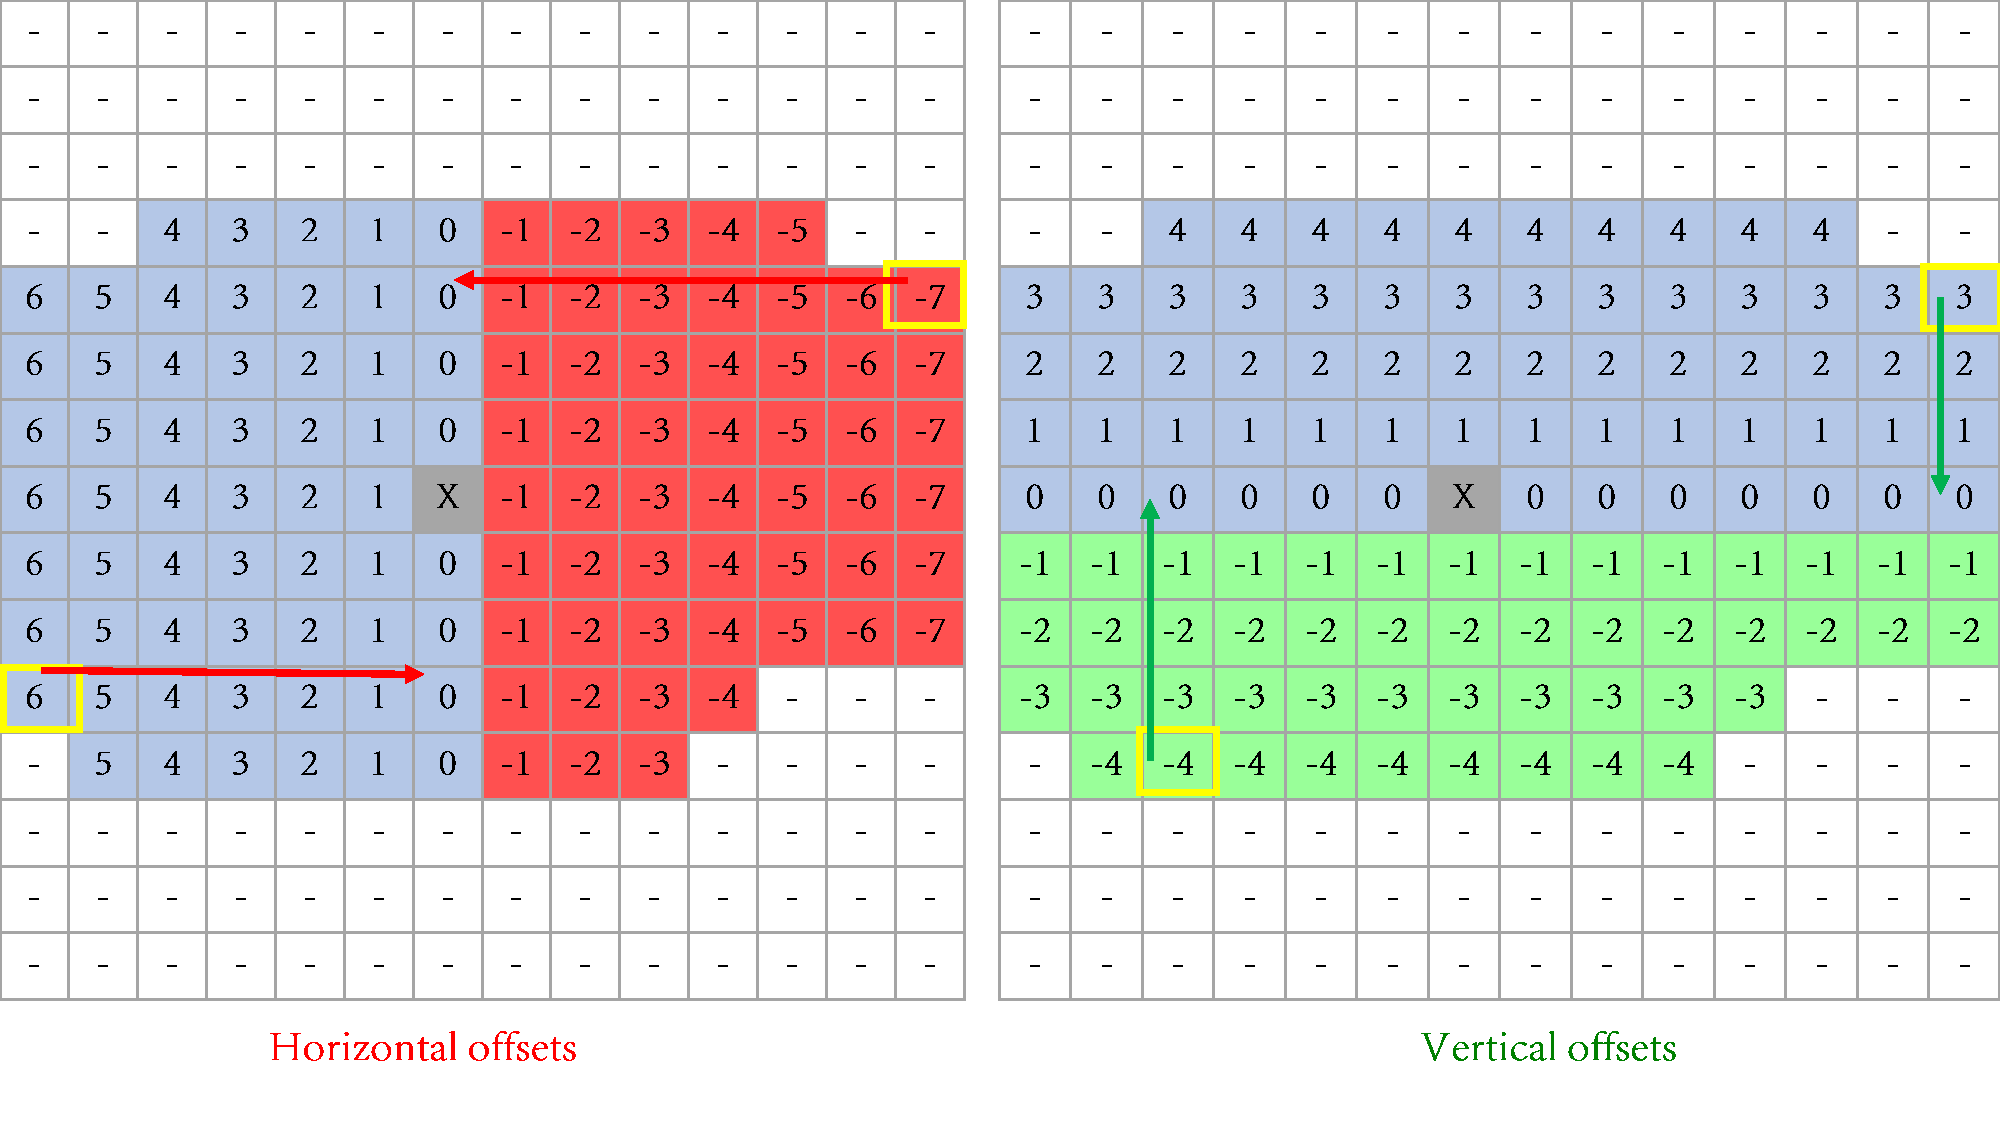
\includegraphics[width = \textwidth]{Graphics/Methodology/extra_offsets.pdf}
    \caption[Offset Vectors with Recovered Direction]{Illustration of offset vectors with recovered directions - recovered direction is based on the center point predictions, where offset vectors in horizontal and vertical offsets are flipped on one side of the predicted center (recovering the real direction of offset required to reach center)}
    \label{fig:offsets_pixels_recovered}
\end{figure}

\subsection{Instance Grouping}
\label{subsec:regression_approach}

First exact center points are achieved using non-maxima suppression as explained in section \ref{subsec:center_rendering}. Given a center point location, pixel values on the right side of center point in horizontal offsets are inverted which corresponds to a negative offset required to reach the center point if the encoding is center to end. Similarly, pixel values below this center point in vertical offsets are inverted to change direction which again indicates that a negative offset in vertical direction is required to reach center point. This is done independently for each center point. After this operation, each pixel in offset representation encodes the actual offset and direction required to reach center. Visualisation of which can be seen from the figure \ref{fig:offsets_pixels_recovered}, where each pixel in either of the offset predictions has corrected directions and essentially points toward center point.


Hence, to generate the instance segmentation output from processed predicted representation, first exact center pixel positions for all center points of potential instances are recovered. And offset vectors are ensured to point correctly in real offset direction i.e, if the encoding is end-to-end, see section \ref{subsec:e2e} - no processing required on the other hand, if encoding is center-to-end as described in section \ref{subsec:c2e} - offset vectors are inverted on one side in both horizontal and vertical offset predictions as illustrated  in figure \ref{fig:c2e_vis_pixels}. The resulting offset predictions then exhibit a predicted offset to their corresponding center pixel with true direction as visualised in figure \ref{fig:offsets_pixels_recovered}.  

\begin{figure}[!ht]
    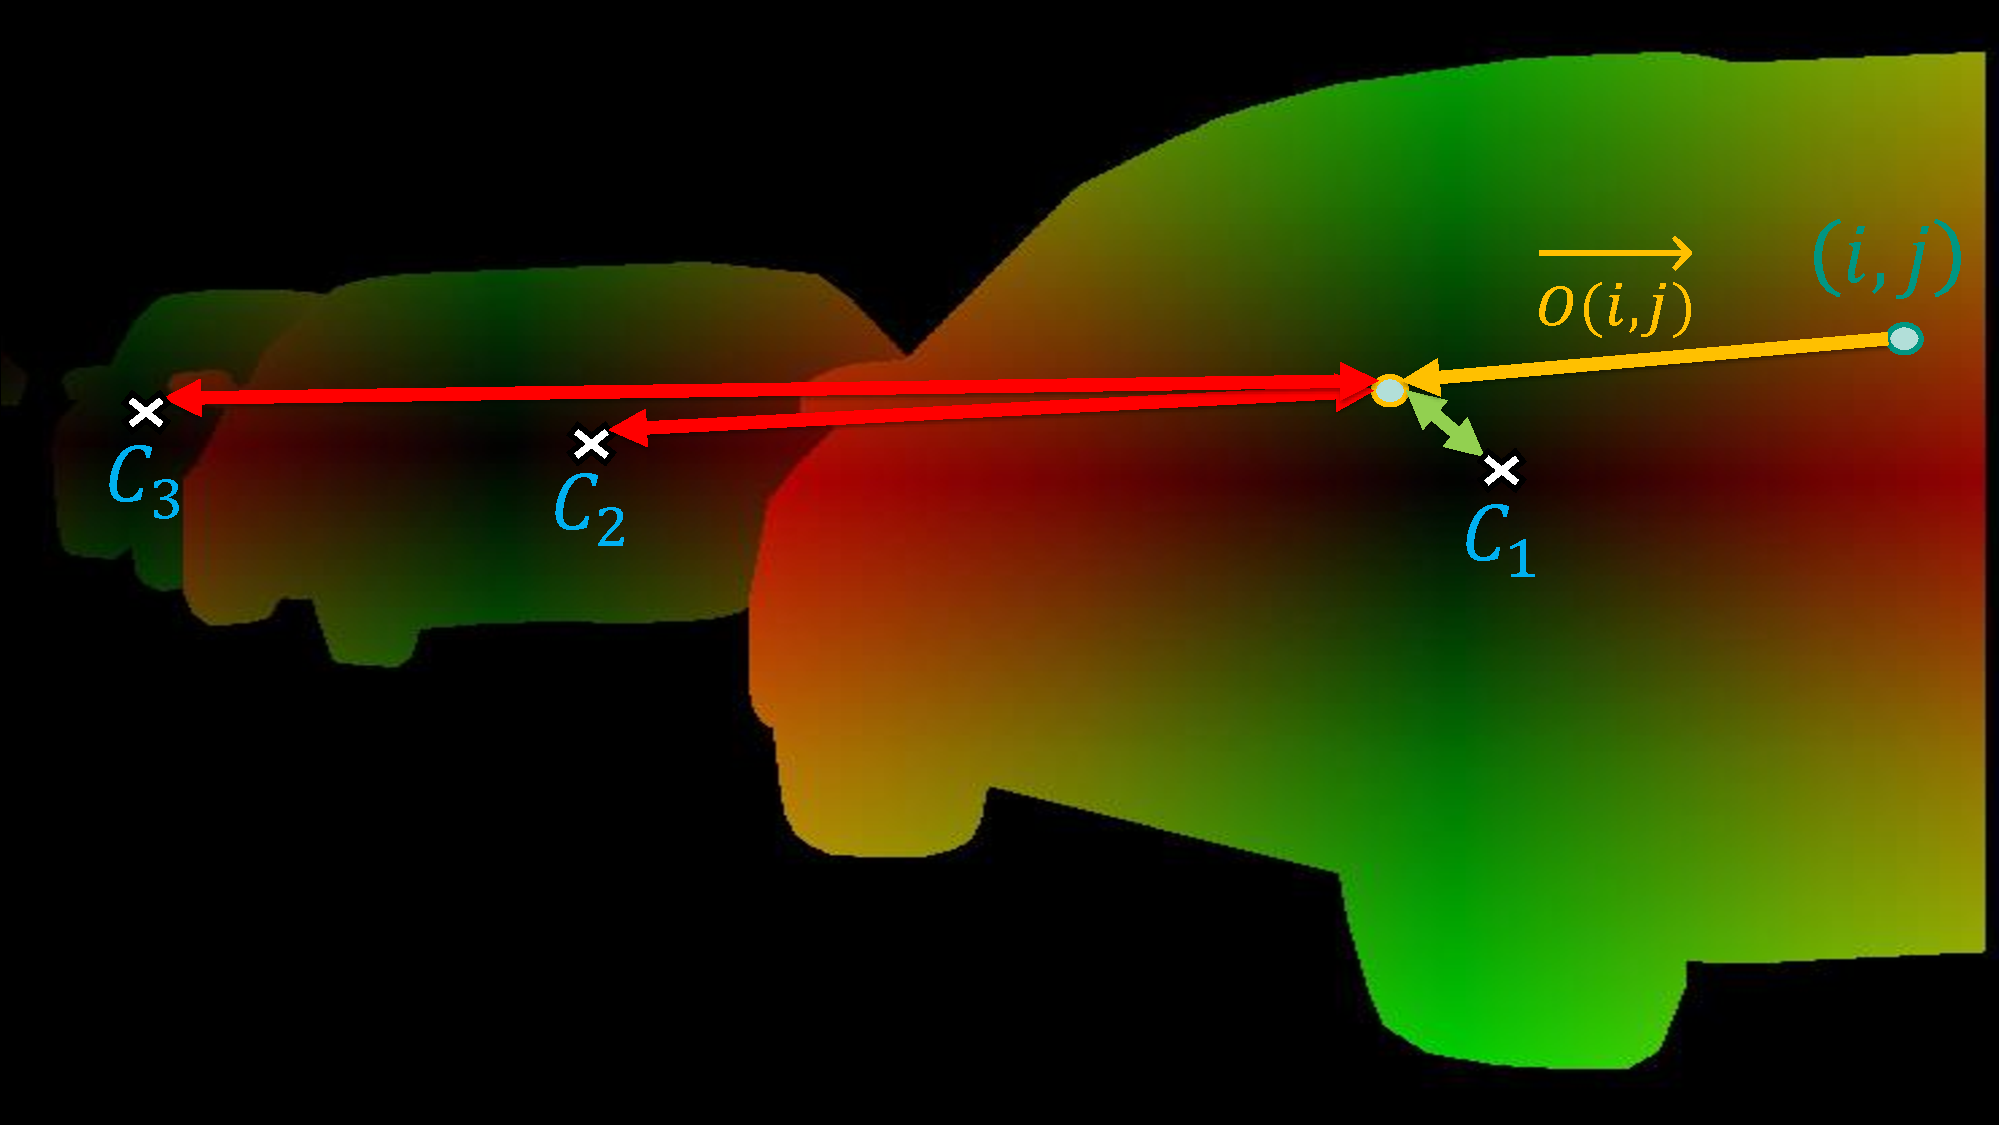
\includegraphics[width = \textwidth]{Graphics/Methodology/instance_regression.pdf}
    \caption[Regression Approach to Generate Instance Masks]{Illustration of regression operation employed to generate instance masks using center point positions and offset vector representations. Given a pixel at position $(i,j)$, it is moved by the predicted offset to a new location. This new location is compared to all the center positions, the pixel in the end is assigned to the center closest to the new location.}
    \label{fig:regression_approach}
\end{figure}

Given the processed representations as described, pixel grouping is then posed as a simple regression problem to generate class-agnostic instance masks as described by equation \ref{eq:regression}, originally proposed by \cite{Deeplabv3+:journals/corr/abs-1802-02611}.

\begin{equation}\hat{k}_{i, j}=\underset{k}{\operatorname{argmin}}\left\|\mathcal{C}_{k}-((i, j)+\mathcal{O}(i, j))\right\|^{2}
\label{eq:regression}
\end{equation}

Consider a pixel location $(i,j)$ as shown in the image \ref{fig:regression_approach}, move the pixel by an offset vector $\mathcal{O}(i,j)$ - which is the resultant vector of two vectors extracted from encoded values in horizontal and vertical offset predictions. Distance of this new position of pixel is calculated with respect to all the center points in the image. Finally, pixel $(i,j)$ is assigned to the center that exhibits least distance to the new position of the pixel. Same approach is taken for all the pixels in the offset predictions resulting in as many instance masks as centers pooled after \gls{nms} - essentially class-agnostic instance segmentation. In the presented work, this regression operation has been implemented as fast and efficient vectorized matrix operations.







\subsection{Panoptic Representation}


Prior sections of this chapter describe simple post-processing steps to generate class-agnostic instance segmentation. In this section, panoptic representation has been explained. The final goal of the task is to generate a representation that is easy to interpret and provides for a detailed information about the scene including semantic layout and instance level information of traffic participants. 

Goal of panoptic segmentation is to assign a unique value to every pixel in the image that encodes both semantic label and instance id.  Given a pixel value - $x_i$ where $\lceil x_i / 1000\rceil$  represents the semantic label, and remainder of $( x_i / 1000 )$ represents instance id.

Few sample encoded values of panoptic segmentation task are: 26000, 260001, 260002, 260003, 19, 18. In the first 3 examples belong to \textit{things class} where 26 is the class label and 0, 1, 2, 3 are instance ids whereas in the last two examples 18, and 19 represent pixels belonging to \textit{stuff} classes.

Therefore, generating a panoptic segmentation label is simple and defined as follows:

\begin{equation}
\mathrm{panoptic_{id}} = \mathrm{1000 class_{id}} + \mathrm{instance_{id}}
\label{eq:outeredgemodel}
\end{equation}


To generate such an encoding, it is important to first assign class labels to class-agnostic instance masks generated by post-processing of instance decoder outputs, as described. Assigning class label is a fast and parallel operation of majority voting implemented on \gls{gpu} where every masked regions is assigned a class label by looking into the same region in semantic segmentation prediction. Final class label is then assigned by simple majority voting for each instance mask which takes about 3ms on \gls{gpu} as suggested by \cite{Cheng_2020_CVPR}.




